%%==========================================================================
%%  saus-slides-demo.tex
%%  Feature tour of the SAUS Beamer theme.
%%  Compile with:  latexmk saus-slides-demo.tex
%%  (.latexmkrc selects LuaLaTeX; `latexmk -xelatex` also works. pdfLaTeX
%%   compiles too, but without Fira Math or Sindhi/Urdu.)
%%==========================================================================
\documentclass[aspectratio=169,11pt]{beamer}

% titlestyle = photo (default) | solid | split
% logo       = corner (default) | none
% numbering  = counter (default) | fraction | none
% native     = sindhi (default) | urdu | both | none
\usetheme[titlestyle=photo]{SAUS}

\usepackage{booktabs}

%% ---- Institutional details (defaults are already the university's) -------
\sausdepartment{Department of Computer Science}
\sausevent{Faculty Development Seminar}

%% ---- Presentation details ------------------------------------------------
\title[Digital Transformation]{Digital Transformation of Campus Services}
\subtitle{A roadmap for the 2026--2029 planning cycle}
\author{Dr.\ A.\ Presenter}
\date{21 September 2026}

\begin{document}

%% ---- Title ---------------------------------------------------------------
\begin{frame}[plain,noframenumbering]
  \titlepage
\end{frame}

%% ---- Outline -------------------------------------------------------------
\begin{frame}{Outline}
  \tableofcontents
\end{frame}

\section{Context}

\begin{frame}{The university at a glance}{Established to revive the educational glory of Shikarpur}
  \begin{columns}[T,onlytextwidth]
    \begin{column}{0.30\textwidth}\sausstat{7}{Degree programmes}\end{column}
    \begin{column}{0.30\textwidth}\sausstat{2}{Faculties}\end{column}
    \begin{column}{0.30\textwidth}\sausstat{815}{Students enrolled}\end{column}
  \end{columns}

  \sausrulesep

  \begin{itemize}
    \item A \sauskey{public sector general university} serving Shikarpur and upper Sindh.
    \item Teaching, research and community engagement across the humanities,
          sciences and professional disciplines.
      \begin{itemize}
        \item Second-level items use the crest's royal blue.
        \item Third-level items pick up the gold accent.
      \end{itemize}
  \end{itemize}
\end{frame}

\begin{frame}{One university, three scripts}{Sindhi in Lateef, Urdu in Nastaliq}
  \renewcommand{\arraystretch}{1.9}
  \begin{tabular}{@{}l@{\hspace{2.5em}}l@{}}
    {\small\color{sausslate}English} & \Large The Shaikh Ayaz University, Shikarpur \\
    {\small\color{sausslate}Sindhi}  & \Large\sausnamesindhi \\
    {\small\color{sausslate}Urdu}    & \Large\sausnameurdu
  \end{tabular}

  \sausrulesep
  \small Use \texttt{\textbackslash sausnamesindhi} and \texttt{\textbackslash sausnameurdu}
  anywhere, or \texttt{\textbackslash saussindhi\{\dots\}} and
  \texttt{\textbackslash sausurdu\{\dots\}} for any phrase.
\end{frame}

\begin{frame}{Blocks and semantic colours}
  \begin{columns}[T,onlytextwidth]
    \begin{column}{0.48\textwidth}
      \begin{block}{Standard block}
        Maroon header on the crest's mist tint. Use for definitions,
        summaries and key takeaways.
      \end{block}
      \begin{exampleblock}{Example block}
        Royal blue header, sampled from the ring of the university crest.
      \end{exampleblock}
    \end{column}
    \begin{column}{0.48\textwidth}
      \begin{alertblock}{Alert block}
        Reserved for deadlines, risks and anything that must not be missed.
      \end{alertblock}
      \begin{block}{Emphasis}
        \sauskey{Key terms} sit in maroon bold; \saushl{highlights} use a
        light gold wash. \alert{Alerted text} is red.
      \end{block}
    \end{column}
  \end{columns}
\end{frame}

\section{Programme of work}

\begin{frame}[plain,noframenumbering]
  \sausstatement{Every service a student touches should work on a phone,
  in Sindhi or English, on the first attempt.}
\end{frame}

\begin{frame}{Numbered workstreams}
  \begin{enumerate}
    \item Student records and admissions portal
    \item Learning management system and lecture capture
    \item Campus network, Wi-Fi and data centre refresh
    \item Library discovery and digital repository
  \end{enumerate}

  \begin{description}
    \item[Phase 1] Assessment and procurement.
    \item[Phase 2] Pilot with two faculties.
    \item[Phase 3] University-wide rollout.
  \end{description}
\end{frame}

\begin{frame}{Tabular data}
  \begin{table}
    \centering
    \begin{tabular}{@{}llr@{}}
      \toprule
      \textbf{Workstream} & \textbf{Owner} & \textbf{Year} \\
      \midrule
      Admissions portal   & Registrar's Office & 2026 \\
      Learning management & Faculty of Education & 2027 \\
      Network refresh     & IT Directorate & 2027 \\
      Digital repository  & Central Library & 2028 \\
      \bottomrule
    \end{tabular}
    \caption{Indicative delivery schedule.}
  \end{table}
\end{frame}

\begin{frame}{Mathematics}{Fira Math is drawn to match the text face}
  Growth in enrolment, modelled as
  \[
    N(t) = N_0\,e^{rt}, \qquad r = \frac{1}{T}\ln\frac{N_T}{N_0}.
  \]
  From $N_0 = 815$ students today to an illustrative $N_T = 1500$ in 3 years,
  $r \approx 0.203$.

  \begin{exampleblock}{Cauchy--Schwarz, in a block}
    \[
      \Bigl(\sum_{i=1}^{n} a_i b_i\Bigr)^{2}
      \le \sum_{i=1}^{n} a_i^{2} \, \sum_{i=1}^{n} b_i^{2}
      \qquad \forall\, a, b \in \mathbb{R}^n
    \]
  \end{exampleblock}
\end{frame}

\section{The campus}

\begin{frame}[plain,noframenumbering]
  \sausphotoslide{assets/saus-campus-gate.jpg}%
    {The campus on Main Road, Shikarpur --- the setting for every service
     described in this plan.}
\end{frame}

\begin{frame}[plain,noframenumbering]
  \sausquote{Revival of Educational Glory of Shikarpur.}%
    {Motto of The Shaikh Ayaz University, Shikarpur}
\end{frame}

\begin{frame}{Figures}
  \begin{columns}[c,onlytextwidth]
    \begin{column}{0.55\textwidth}
      \begin{figure}
        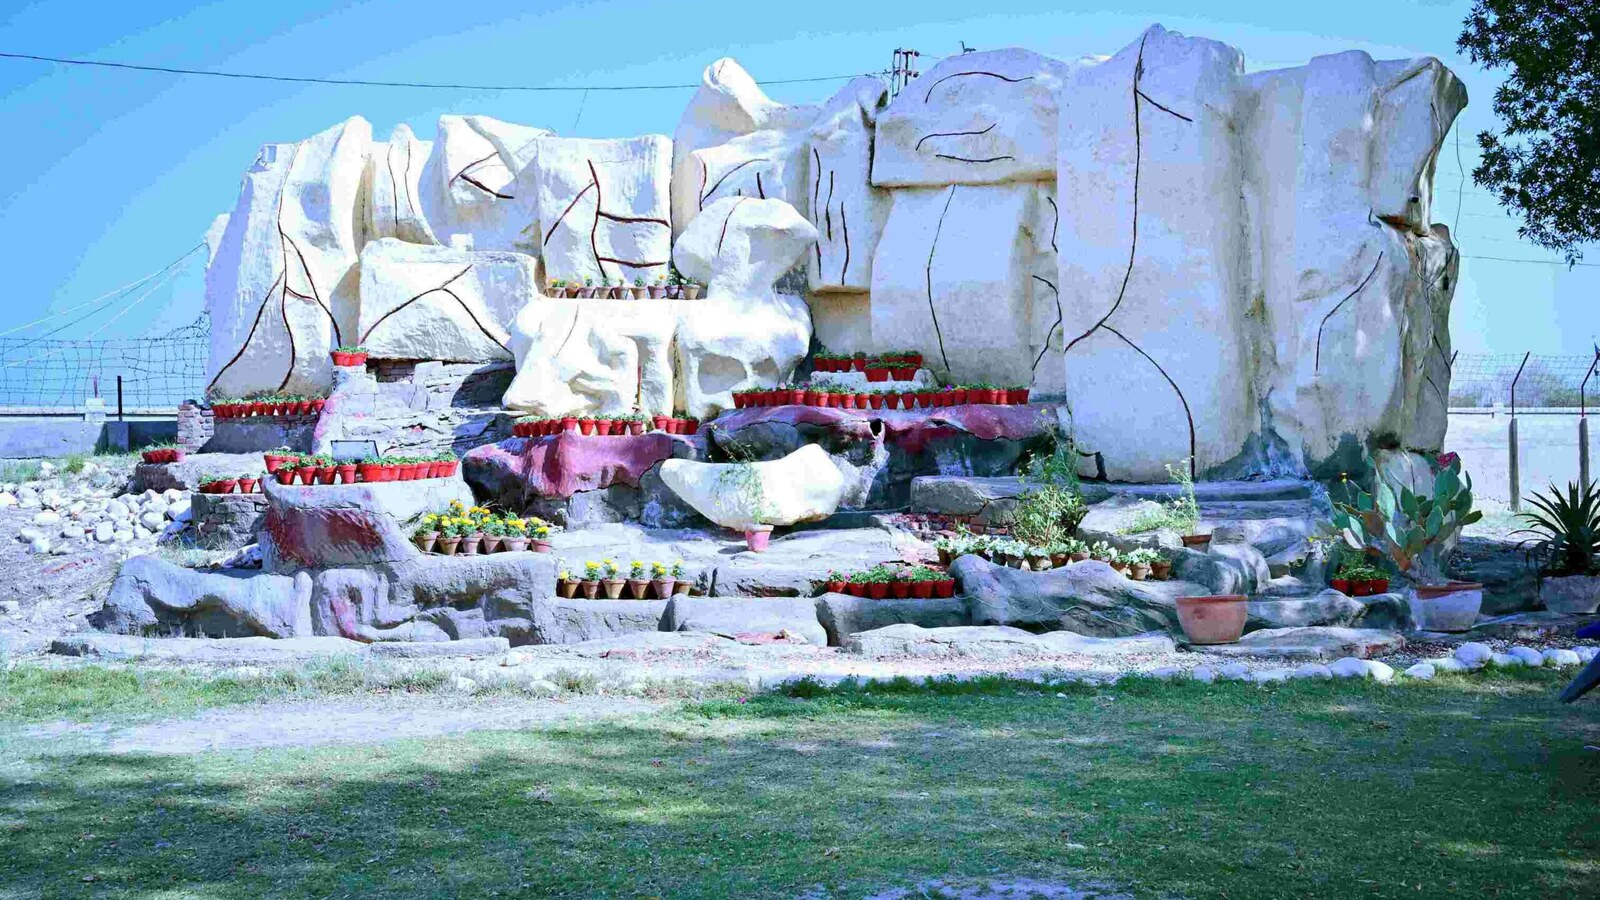
\includegraphics[width=\linewidth]{assets/saus-monument.jpg}
        \caption{The campus monument.}
      \end{figure}
    \end{column}
    \begin{column}{0.41\textwidth}
      Captions are numbered and the label is set in maroon.
      \medskip

      Photographs sit flush to the text column; full-bleed images get their
      own slide with \texttt{\textbackslash sausphotoslide}.
    \end{column}
  \end{columns}
\end{frame}

%% ---- Closing -------------------------------------------------------------
\begin{frame}[plain,noframenumbering]
  \sausthankyou
\end{frame}

\end{document}
